\paragraph{Sơ đồ tuần tự luồng xem và cập nhật tên hiển thị}

Luồng nghiệp vụ này mô tả
quy trình người dùng
tải thông tin cá nhân
và cập nhật tên hiển thị thông qua Auth Service (Supabase).

\begin{figure}[H]
\centering
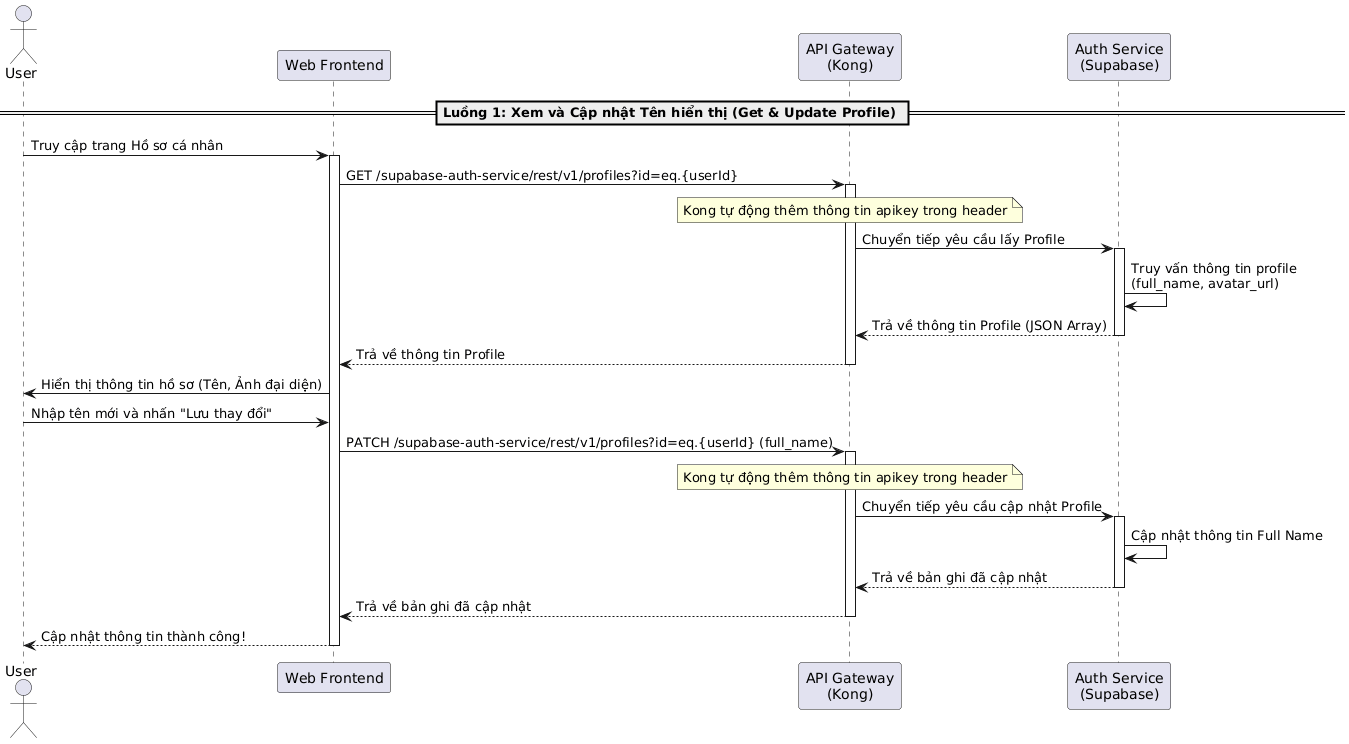
\includegraphics[width=0.95\textwidth]{contents/Sequence/UML-Sequence-UserProfileUpdateDisplayName.png}
\caption{Sơ đồ tuần tự luồng xem và cập nhật tên hiển thị}
\end{figure}

\begin{table}[H]
\centering
\renewcommand{\arraystretch}{1.3}

\begin{tabular}{|l|l|p{5cm}|}
\hline
\textbf{Thành phần} & \textbf{Phân loại} & \textbf{Vai trò trong hệ thống} \\ \hline
User & Actor & Người dùng xem và thay đổi thông tin cá nhân. \\ \hline
Web Frontend & Component & Giao diện web Next.js. \\ \hline
API Gateway (Kong) & Component & Cổng API chuyển tiếp các yêu cầu API. \\ \hline
Auth Service (Supabase) & Component & Dịch vụ thực hiện xác thực, truy vấn và cập nhật thông tin hồ sơ trong CSDL. \\ \hline
\end{tabular}
\caption{Các thành phần tham gia luồng xem và cập nhật tên hiển thị}
\end{table}
\subparagraph{Mô tả tổng quan}

\begin{itemize}

\item \textbf{Tải thông tin hiện tại:}
Người dùng truy cập
trang thông tin cá nhân.
Giao diện gửi yêu cầu lấy thông tin chi tiết của người dùng qua cổng API
dựa trên định danh tài khoản.

\item \textbf{Cập nhật tên hiển thị:}
Người dùng nhập tên hiển thị mới và nhấn lưu.
Giao diện gửi yêu cầu cập nhật tên hiển thị mới qua cổng API tới Auth Service để ghi nhận thay đổi.
\end{itemize}
